\section{Block Level Description} \label{sec:block_level}
This section contains block level descriptions of all parts of the system seen in figure \ref{fig:top_level}.

\begin{figure}[H]
  \centering
  \captionsetup{justification=centering}
  \todo{Bild på top level}
  \caption{Block diagram of the system.} \label{fig:top_level}
\end{figure}


\subsection{SPI\_in/PSBR}
The SPI\_in module consists of a lot of registers and some control logic moving data between these registers. Since the PRBS module share some registers with the SPI\_in module, and the PRBS module is relatively small, we included it in the SPI\_in module. \\
The first block in the SPI\_in module is the SPI\_recieve block. It consists of 16 resettable D flip-flops (DFFSR), that is connected one after another. They are clocked on the SPI clock, and on each positive clock pulse, we got a new bit to shift in. After 16 pulses we have 16 bits stored, and a load signal is triggered so that each bit is moved to the correct PRBS-register. \\
The PRBS-registers are register that consists of four DFFSR (one for each addition) and that can be run in two different modes. During the first mode, the normal mode, the registers are triggered with a load signal, and the data to the first DFFSR comes from the SPI\_recieve block. During the second mode, the PRBS mode, the registers and triggered with the system clock, and the data to the first DFFSR is the value of the third and forth DFFSR passed trhough a XOR. The mode is choosen by the SPI\_enable signal.

\subsection{16-bit Kogge-Stone Adder}
The Kogge-Stone adder consists of four simple blocks connected in a complex way, as can be seen in \ref{fig:ks_block}. These four blocks can be seen in figure \ref{fig:red}-\ref{fig:sum}. The red block constitute the initial stage which takes two binary numbers $A$ and $B$ as input. The corresponding truth table is found in table \ref{tab:red} in appendix \ref{app:ks_truth}. The output signals $P$ and $G$ generated from this block are later used by other blocks in the adder. The $G$, also called the Generate signal, trickles down through the hierarchy of yellow, and yellow carry blocks to finally end up in the sum block. The truth table for this block can be found in table \ref{tab:sum}. Truth tables for the yellow and yellow carry blocks are found in table \ref{tab:yellow} and \ref{tab:yellowcarry}.

\begin{figure}[H]
  \centering
  \captionsetup{justification=centering}
  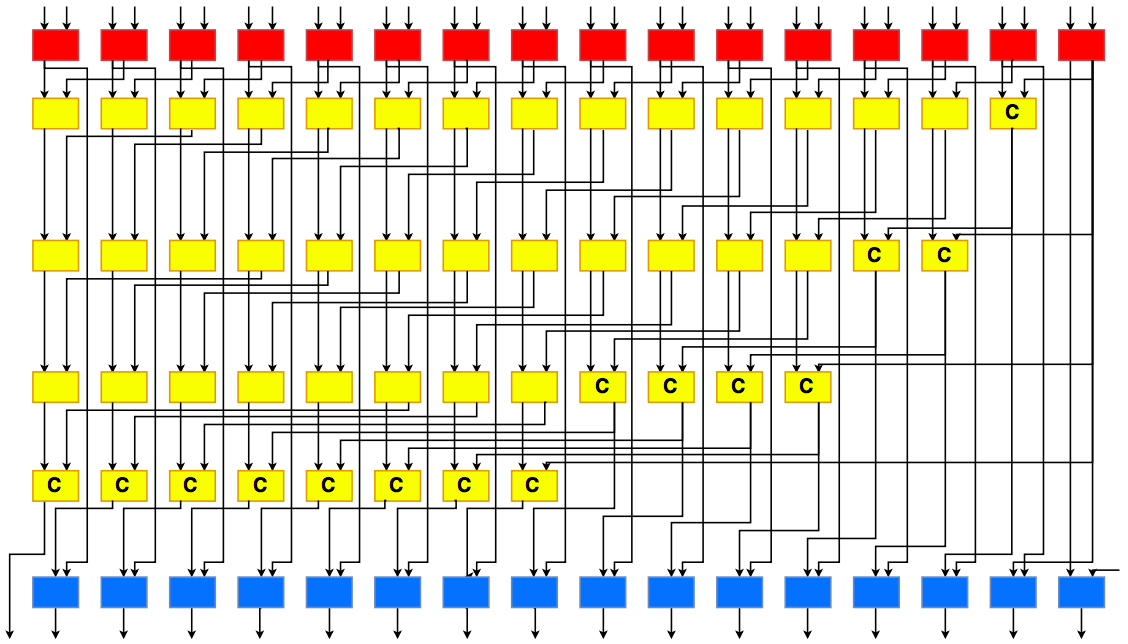
\includegraphics[scale=0.5, angle=90]{../figures/ks_block}
  \caption{Block diagram of the Kogge-Stone Adder.} \label{fig:ks_block}
\end{figure}

\begin{figure}[H]
  \centering
  \captionsetup{justification=centering}
  \adjustbox{trim={.3\width} {0\height} {.3\width} {0\height},clip}
  {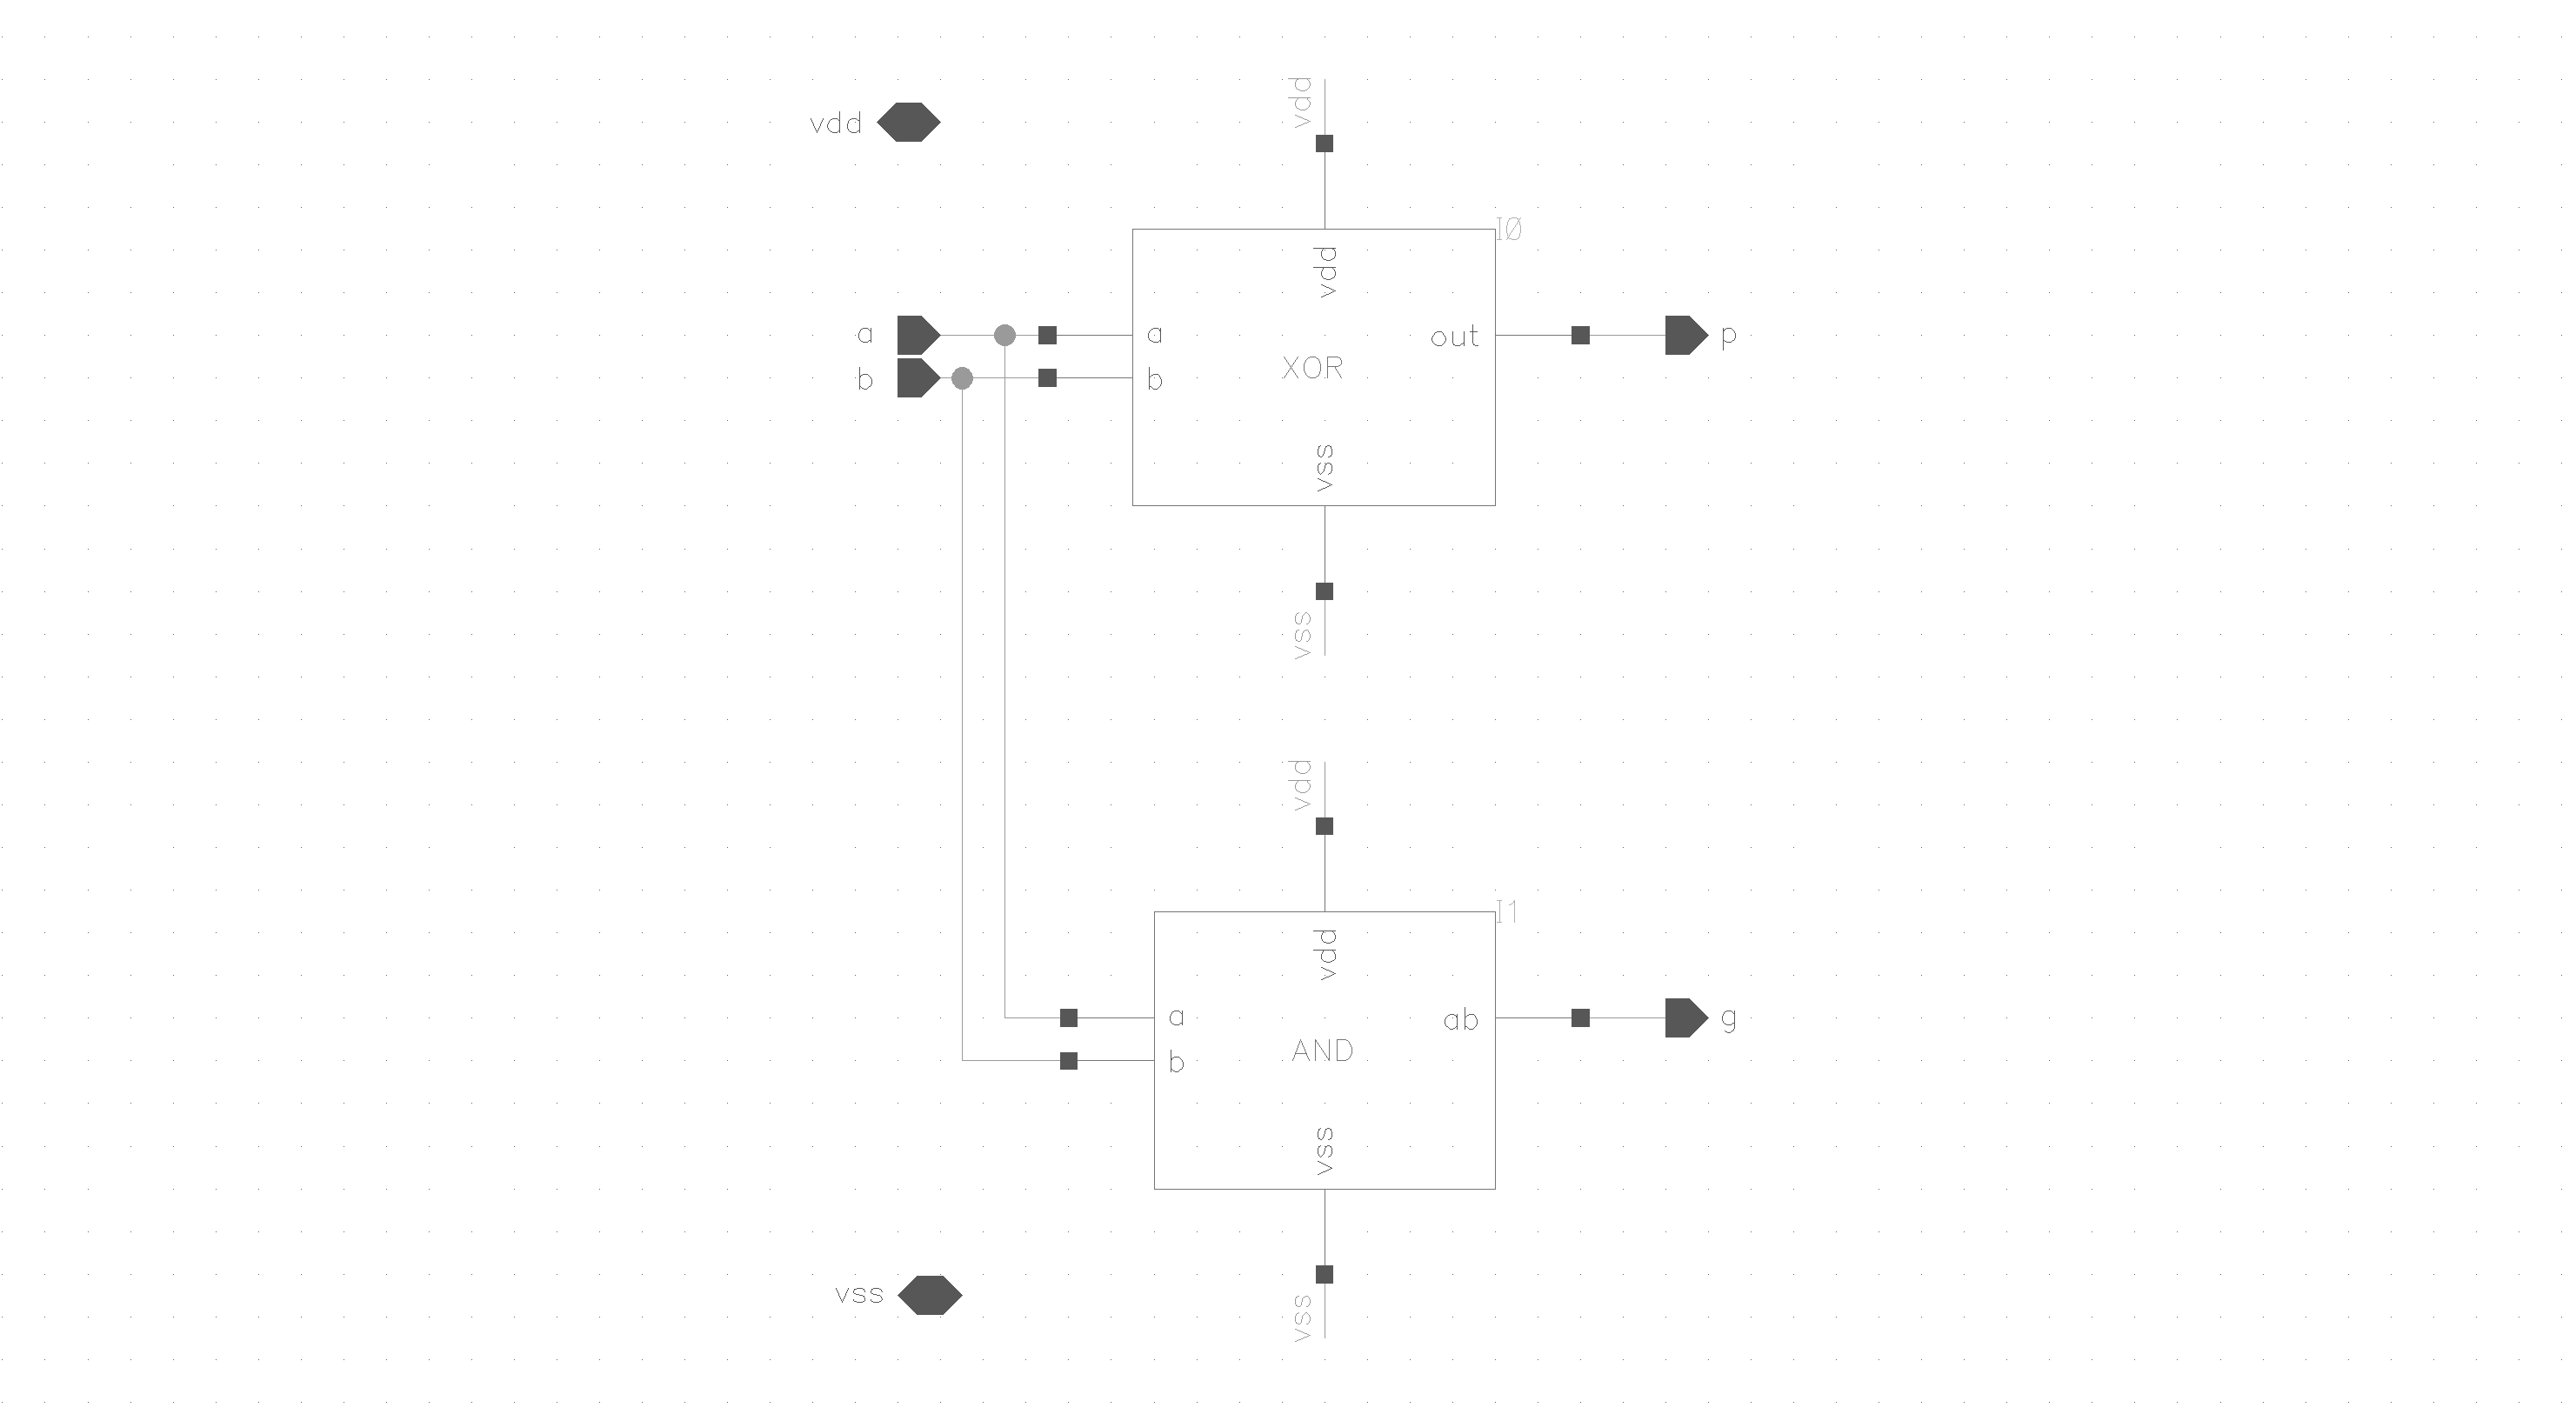
\includegraphics[width=2.0\textwidth]{../figures/red}}
  \caption{Schematic view of the red block.} \label{fig:red}
\end{figure}

\begin{figure}[H]
  \centering
  \captionsetup{justification=centering}
  \adjustbox{trim={.15\width} {0\height} {.12\width} {0\height},clip}
  {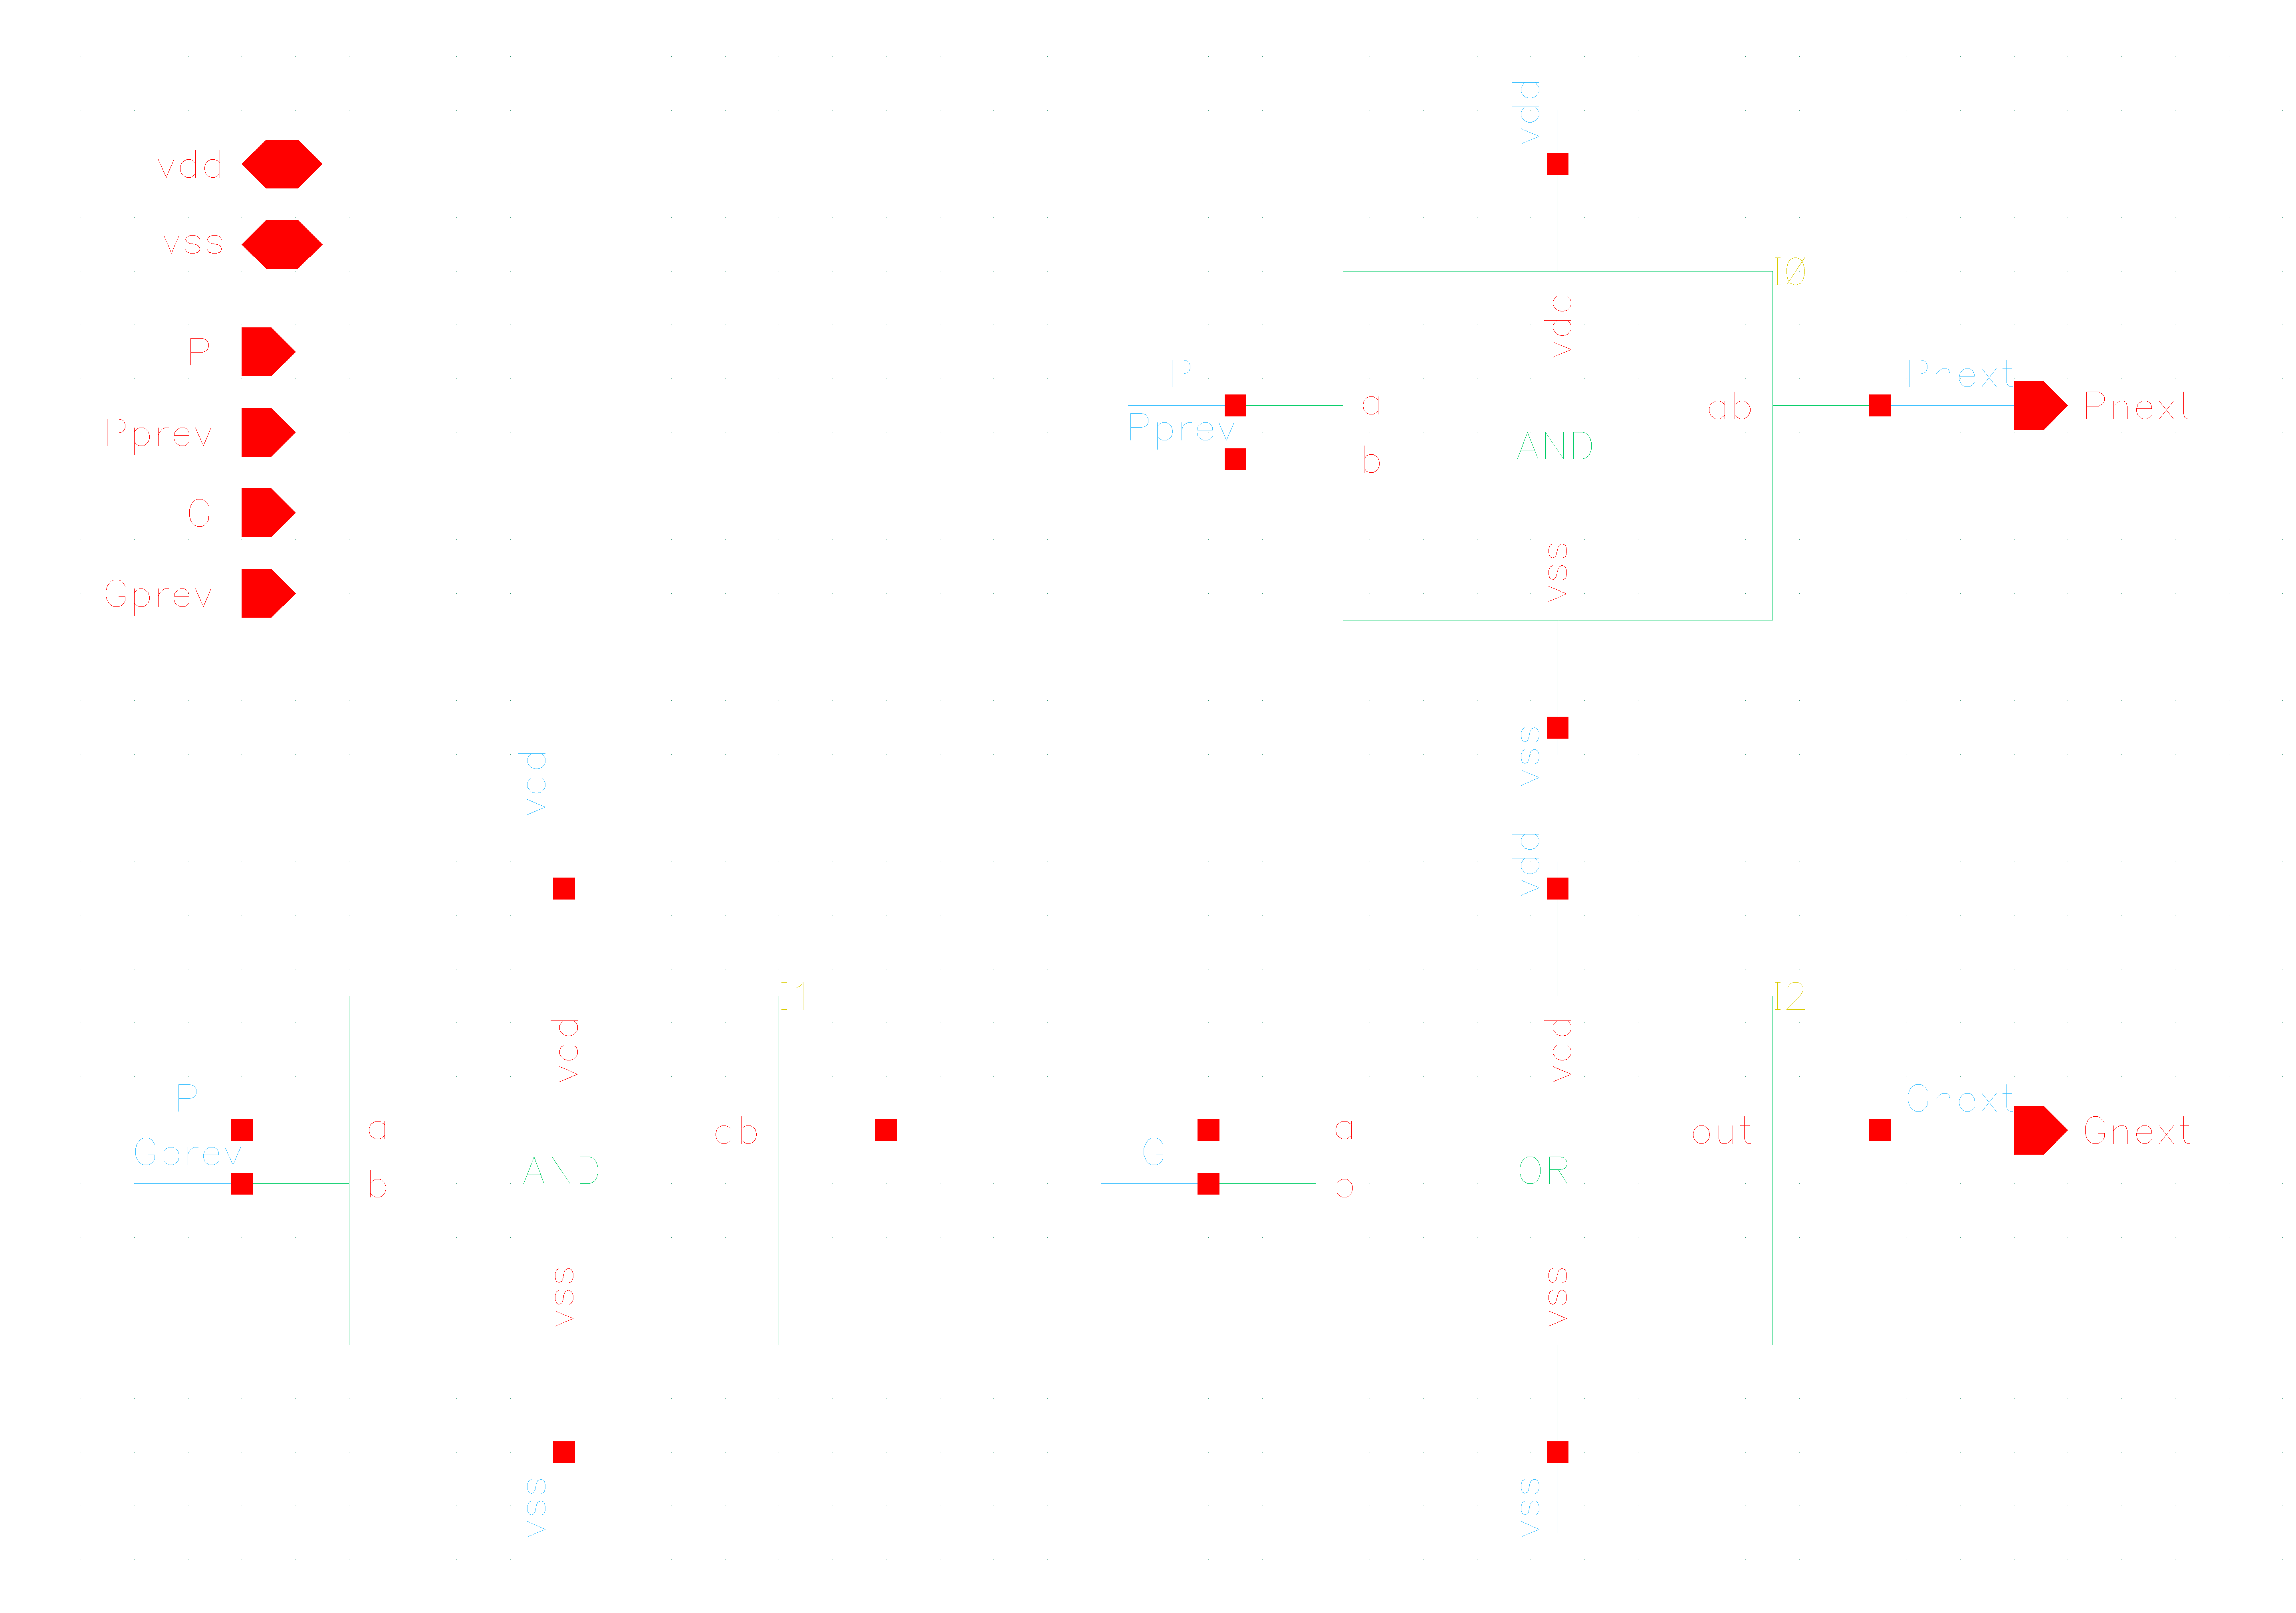
\includegraphics[width=1.3\textwidth]{../figures/yellow}}
  \caption{Schematic view of the yellow block.} \label{fig:yellow}
\end{figure}

\begin{figure}[H]
  \centering
  \captionsetup{justification=centering}
  \adjustbox{trim={.1\width} {0\height} {.1\width} {.4\height},clip}
  {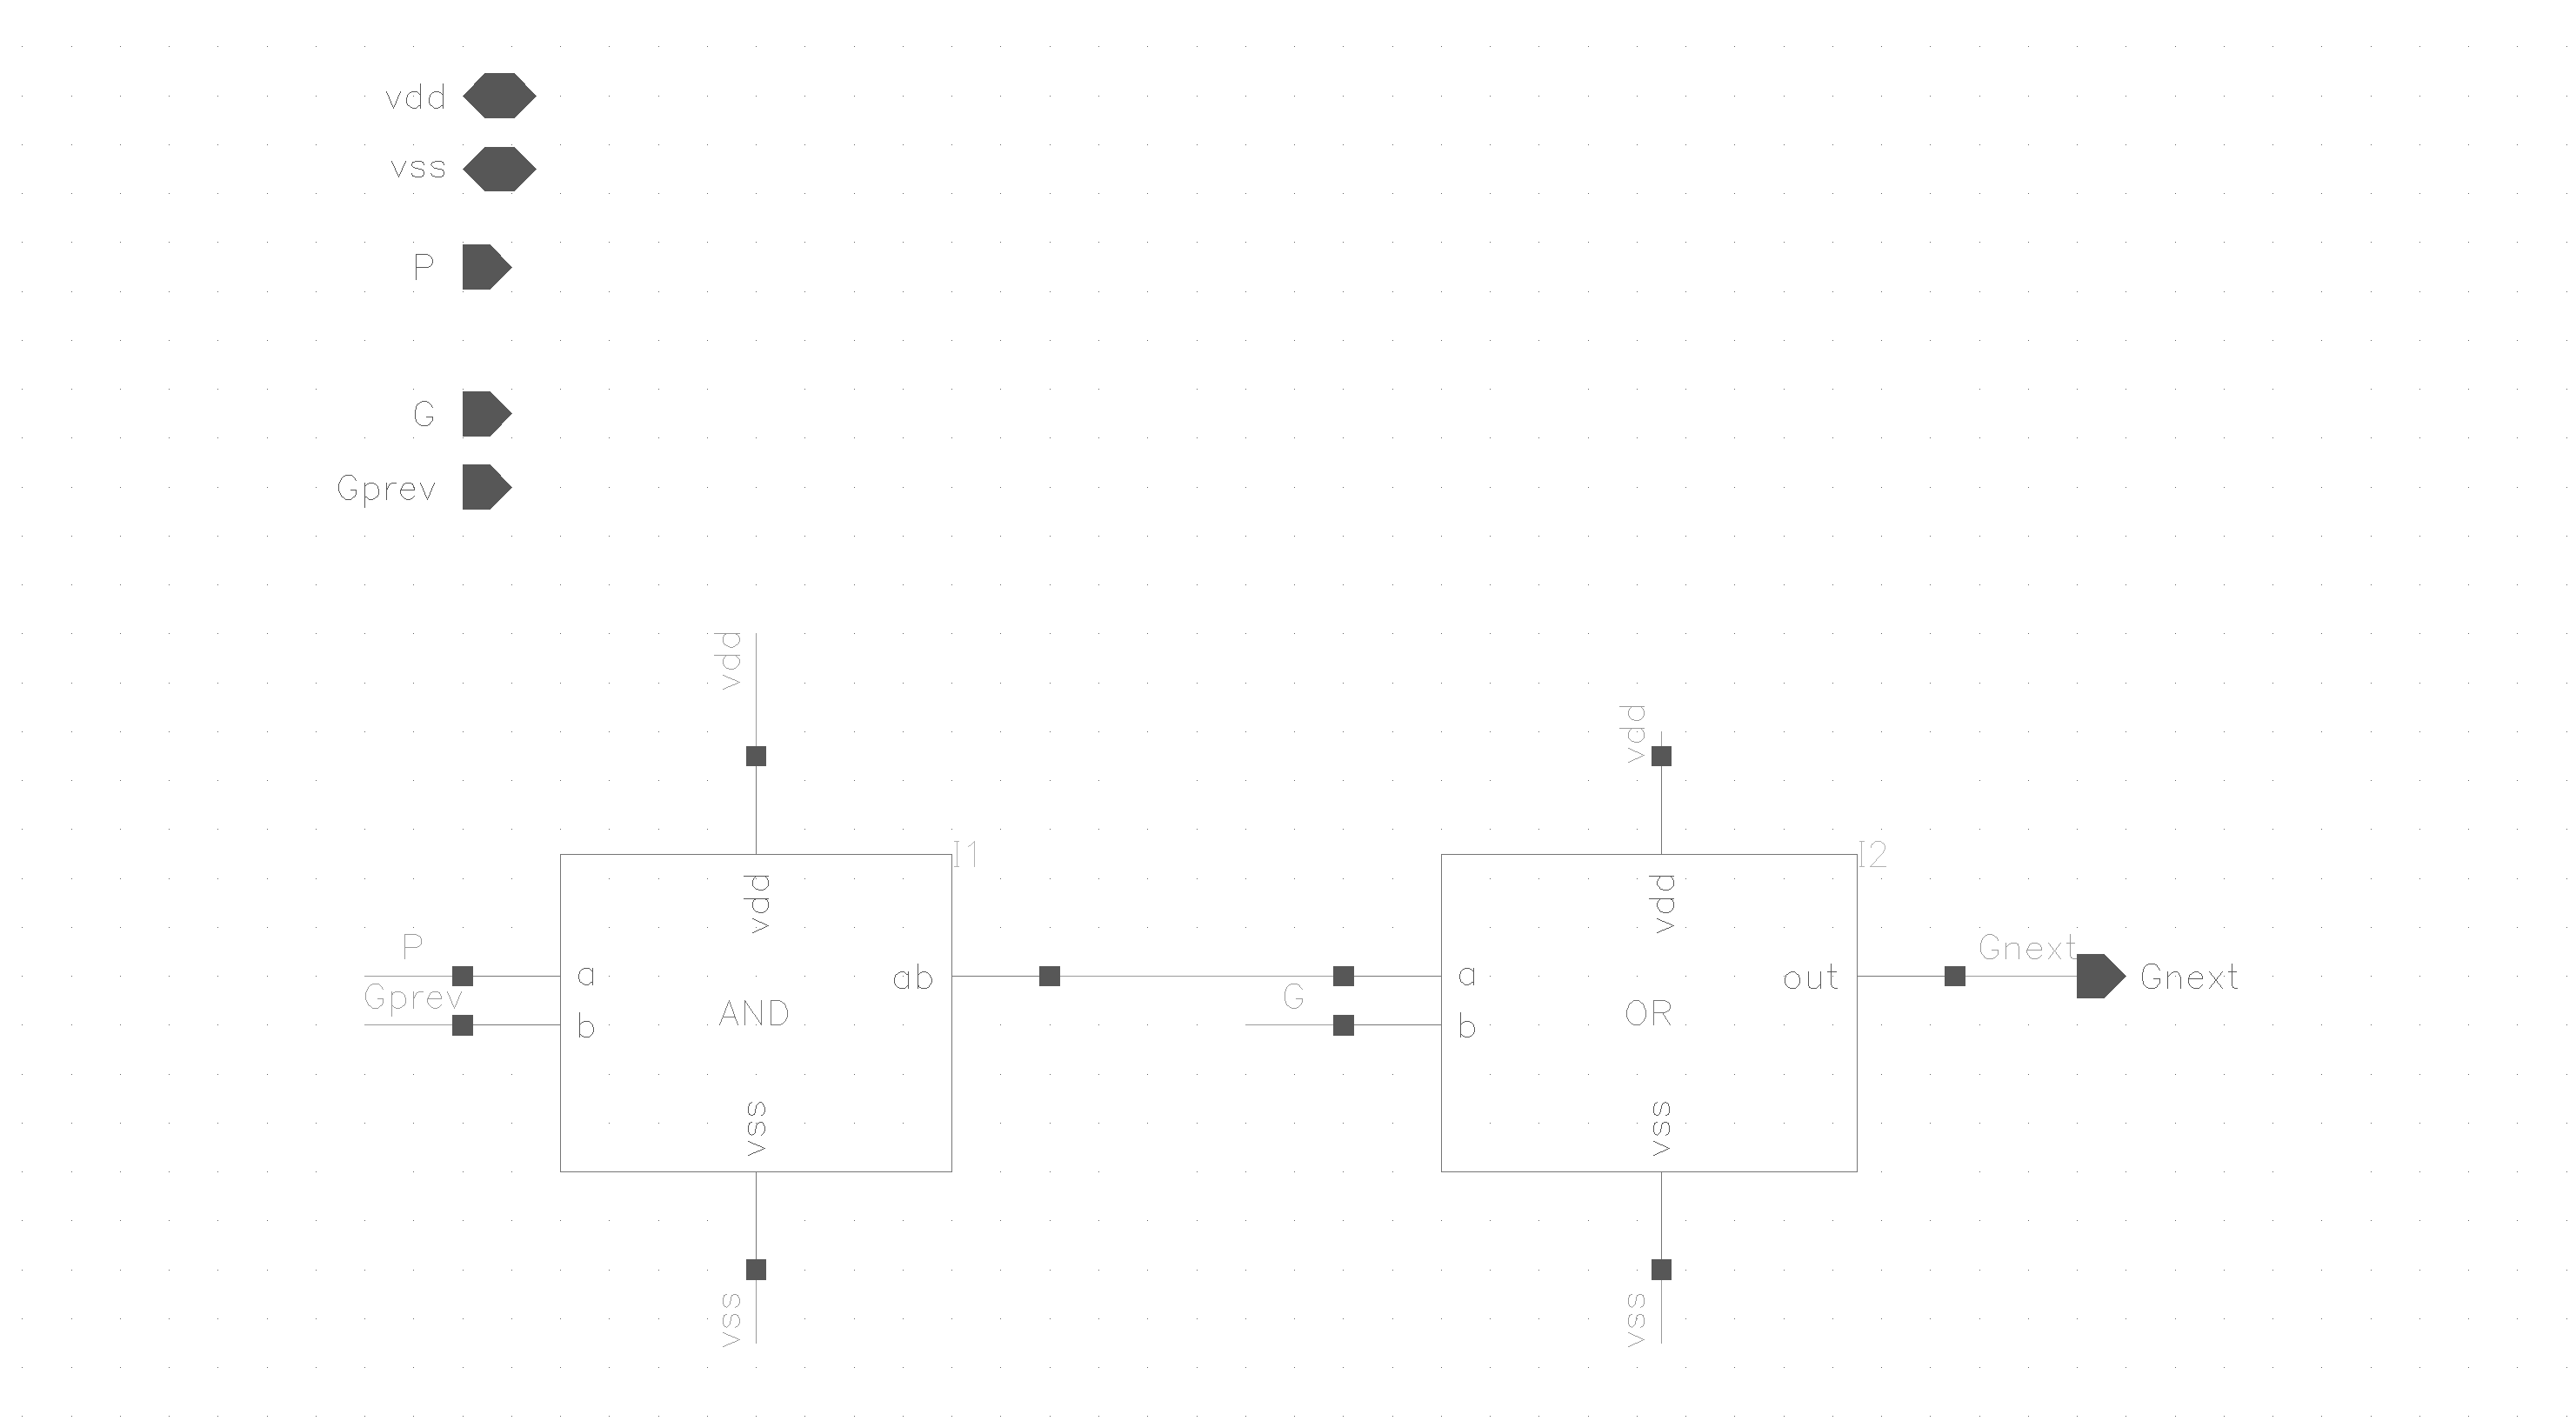
\includegraphics[width=1.2\textwidth]{../figures/yellow_carry}}
  \caption{Schematic view of the yellow carry block.} \label{fig:yellow_c}
\end{figure}

\begin{figure}[H]
  \centering
  \captionsetup{justification=centering}
  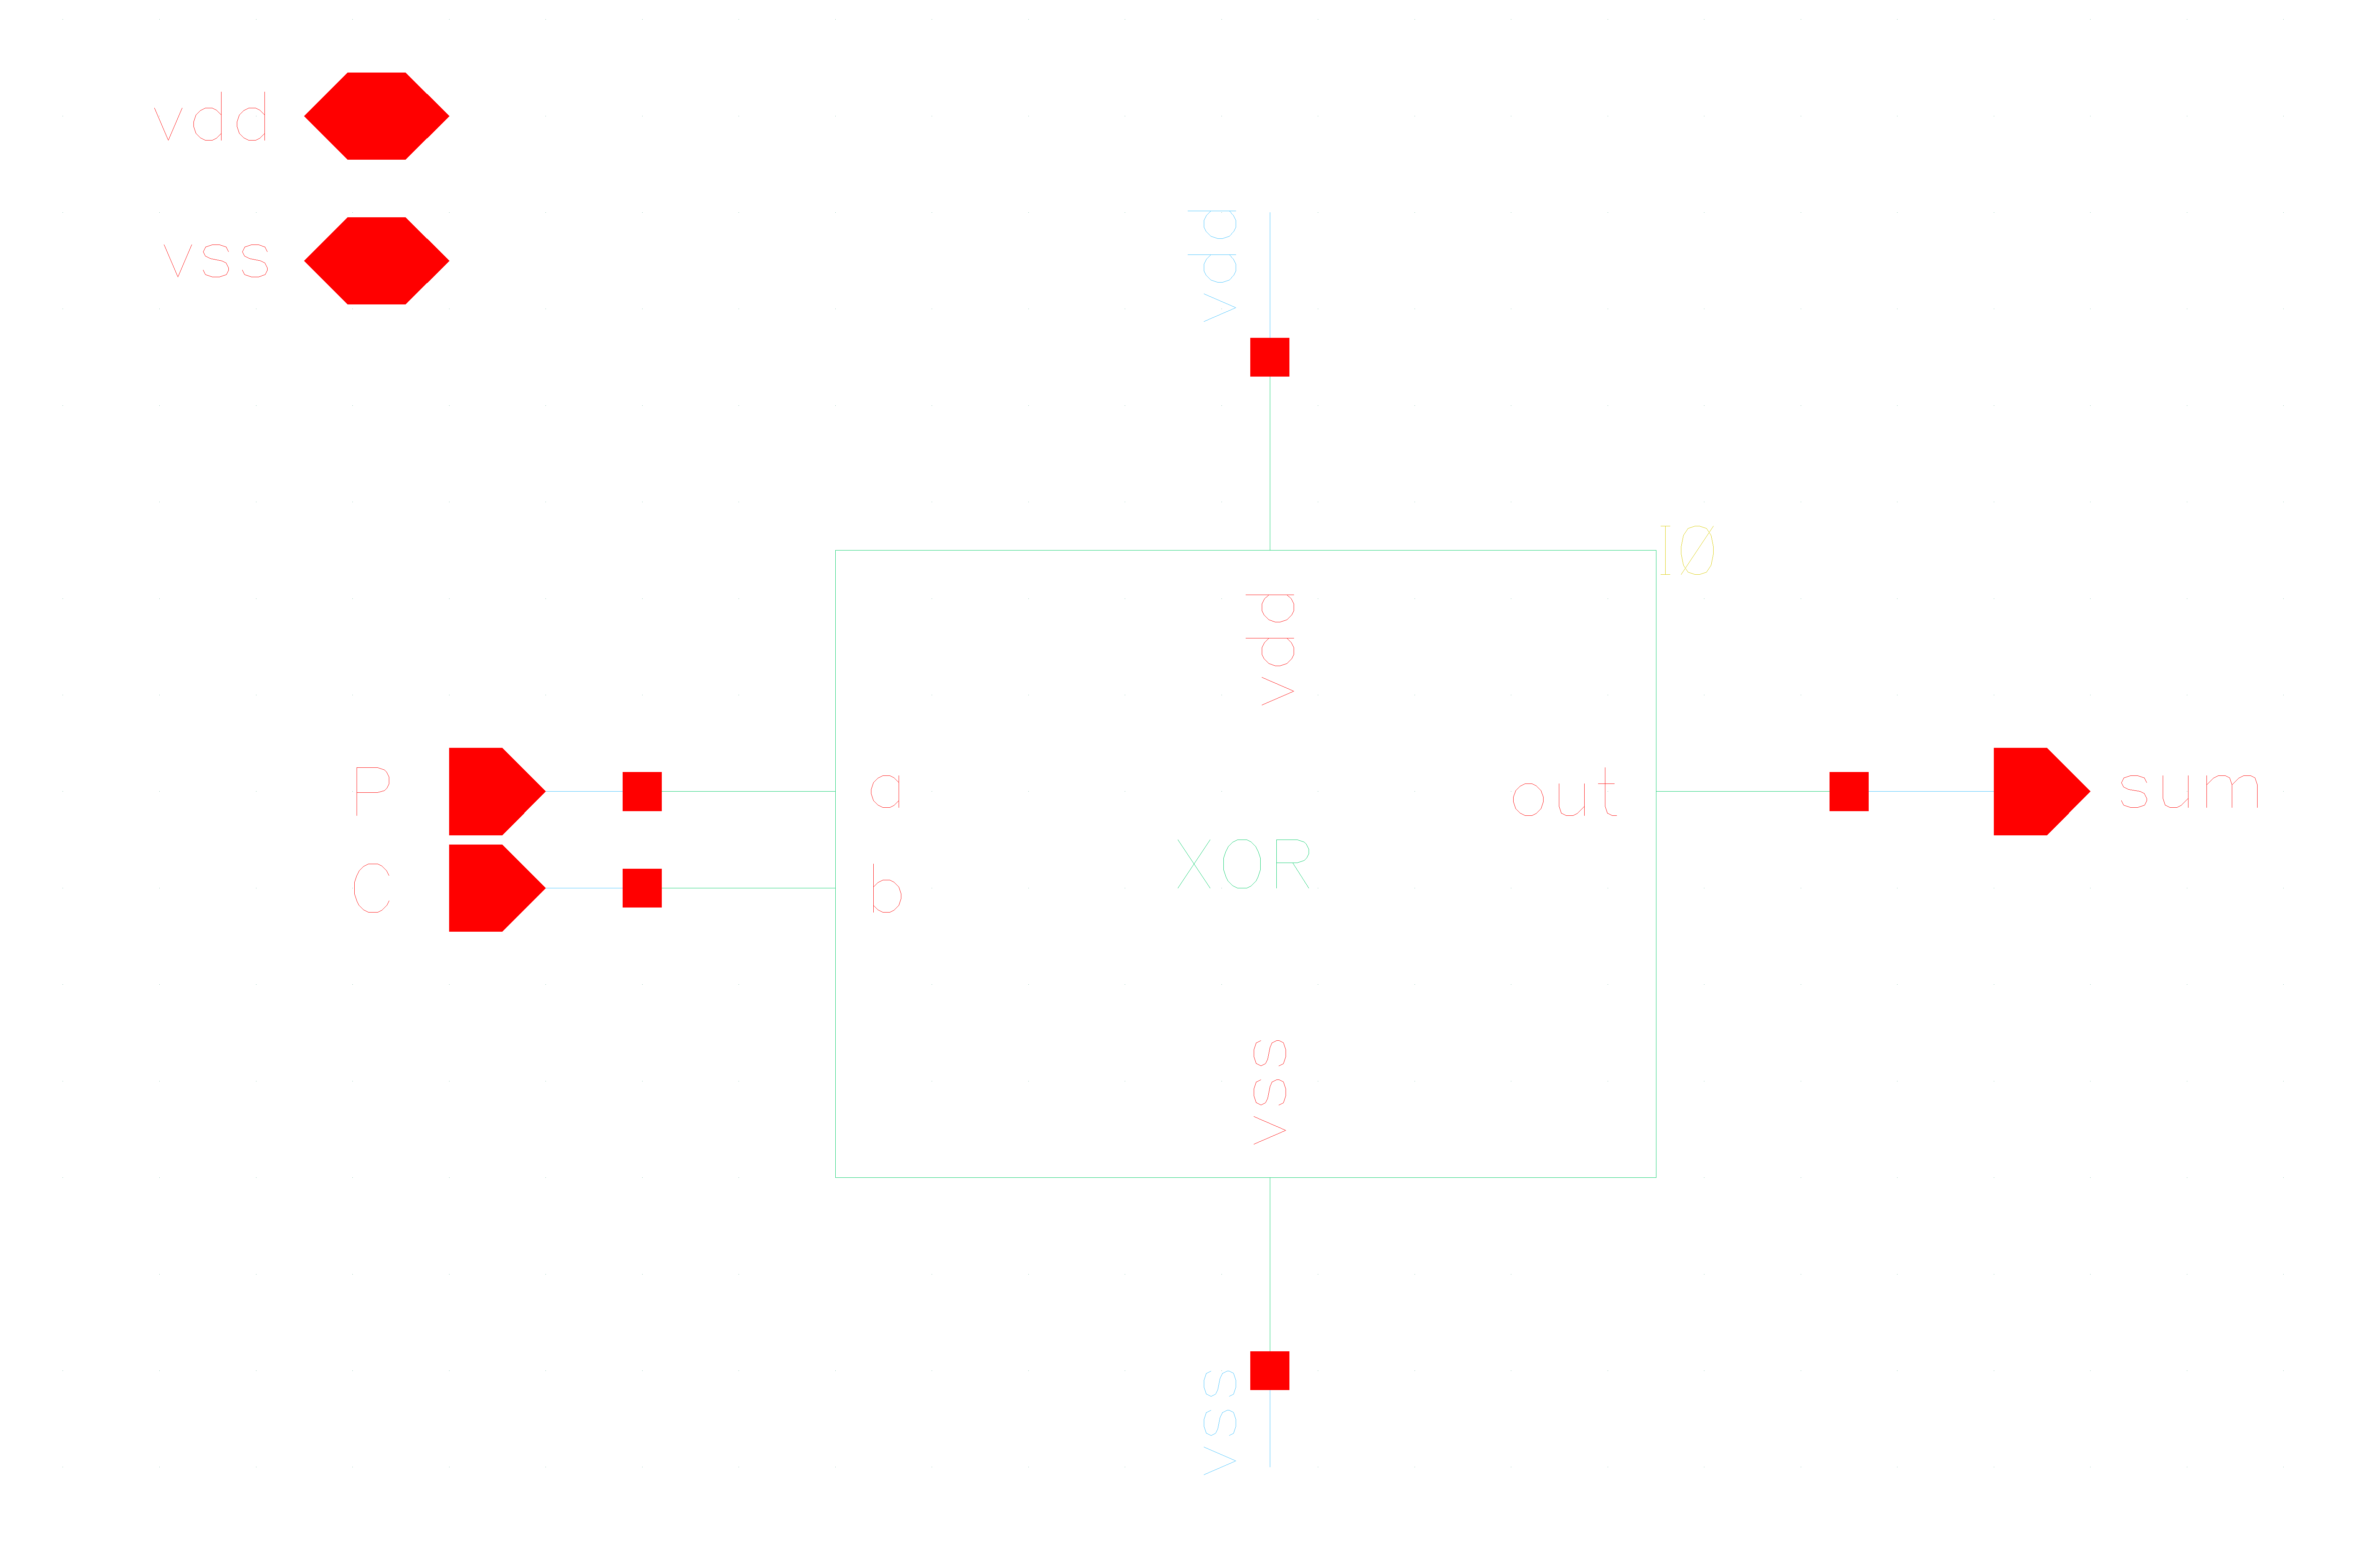
\includegraphics[clip,width=1.0\textwidth]{../figures/sum}
  \caption{Schematic view of the sum block.} \label{fig:sum}
\end{figure}

\subsection{Comparator}
The comparator consists of 17 2-input XNOR gates where one bit of each number is fed into each gate. The output from the XNOR gates are fed into a couple of AND gates which generates the final output. The comparator is 17 bits wide since it compares two 16 bit numbers plus their carry bits. The logic table of the XNOR gates is shown in table \ref{tab:xnor}.

\begin{table}[H]
  \caption{Logic table of XNOR block.}
  \centering
  \begin{tabular}{cc|c}
    \toprule
    $A_i$ & $B_i$ & $Y = \overline{(A_i \oplus B_i)}$ \\
    \midrule
    0 & 0 & 1 \\
    0 & 1 & 0 \\
    1 & 0 & 0 \\
    1 & 1 & 1 \\
    \bottomrule
    \label{tab:xnor}
  \end{tabular}
\end{table}
